\documentclass[a4paper, 12pt]{article}
\usepackage[utf8]{inputenc}
\usepackage[brazil]{babel}
\usepackage{amstext} 	% need for \text command
\usepackage{amsmath}    % need for subequations
\usepackage{amssymb}
\usepackage{graphicx}   % need for figures
\usepackage{verbatim}   % useful for program listings
\usepackage{color}      % use if color is used in text
\usepackage{subfigure}  % use for side-by-side figures
\usepackage{hyperref}   % use for hypertext links, including those to external documents and URLs
\usepackage{pictexwd}	% use for pictex graphs
\usepackage{booktabs}	% use for Publication quality tables in LaTeX

%\author{Vítor M. Martins}
\title{PMR2370}

\begin{document}
\maketitle
%\newpage
%\tableofcontents
%\newpage

\section{Equações}

\paragraph*{Goodman}
\begin{equation}
\frac{\eta \sigma _{a}}{\sigma _{f}}+\frac{\eta \sigma _{m}}{\sigma _{t}}=1
\end{equation}

\paragraph*{ASME}
\begin{equation}
\left( \frac{\eta \sigma _{a}}{\sigma _{f}} \right)^{2}+ \left(  \frac{\eta \sigma _{m}}{\sigma _{esc}} \right)^{2} = 1
\end{equation}


\paragraph*{Gerber}
\begin{equation}
\left( \frac{\eta \sigma _{a}}{\sigma _{f}} \right)^{2}+ \left(  \frac{\eta \sigma _{m}}{\sigma _{t}} \right)^{2} = 1
\end{equation}

\begin{figure}[h]
\begin{center}
\includegraphics[scale=0.38]{./fig/9.png}
\caption{\label{fig:9}} 
\end{center}
\end{figure}

\section{Dano Cumulativo}
Palmgren - Miner

\[\sum _{i=1}^{m} {\frac{n_{i}}{N_{i}}}=1\]

\begin{figure}[h]
\begin{center}
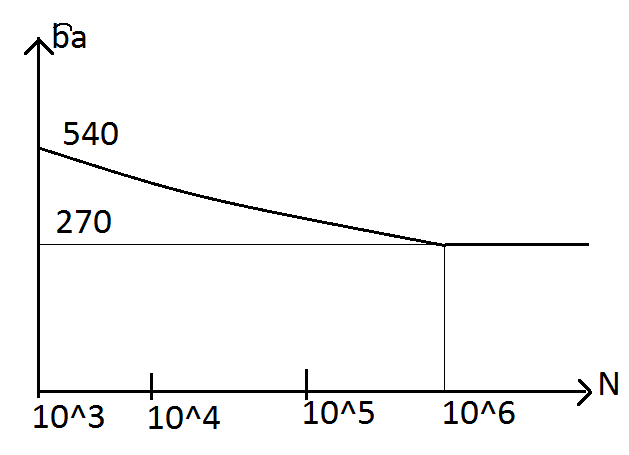
\includegraphics[scale=0.55]{./fig/10.png}
\caption{\label{fig:10}} 
\end{center}
\end{figure}

n = 3000 ciclos @ 480 MPa

\[\sigma _{a}=540-\frac{(540-270)}{3}\left[ \log(N)-3 \right]\]

\newpage

\section{Enunciado}

\begin{figure}[h]
\begin{center}
\includegraphics[scale=0.47]{./fig/Transmissao.png}
\caption{\label{fig:11}Transmissão} 
\end{center}
\end{figure}

\[F_{r}=F_{T}\tan(\alpha)\]
\[ECDR\]
\[\alpha = 20º\]
\begin{itemize}
\item $\sigma _{t}$=630 MPa\ \ \ \ \ \ \ \ \ \ $\sigma _{esc}$=420 MPa
\item confiança 99\%
\item Acoplamento Superficial: retificado / torneado
\item R = 1 mm \ \ \ \ \ \ \ \ \ \ N = 66 W \ \ \ \ \ \ \ \ \ \ n = 600 rpm
\end{itemize}

\subsection*{Solução}
\[N = M_{t}\omega\]
\[6 = M_{t}\frac{600 \pi}{30}\]
\[M_{t}=95 Nm\]
\\
\[F_{T,A}=\frac{M_{t}}{d_{A}/2}=\frac{95}{0.15/2}=1267 N\]
\[F_{T,B}=\frac{M_{t}}{d_{B}/2}=\frac{95}{0.21/2}=905 N\]
\[F_{R,A}=F_{T,A}\tan(\alpha)=461 N\]
\[F_{R,B}=F_{T,B}\tan(\alpha)=329 N\]



\begin{figure}[h]
\begin{center}
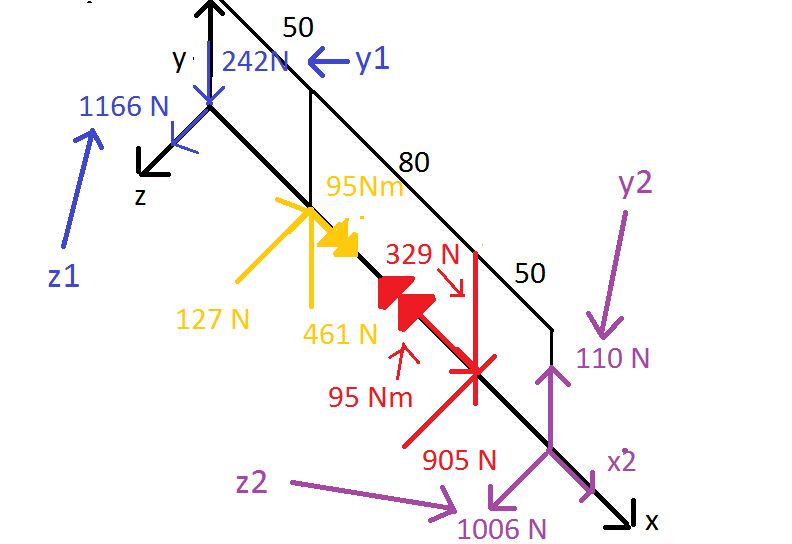
\includegraphics[scale=0.68]{./fig/1.png}
\caption{\label{fig:1}1} 
\end{center}
\end{figure}


\[\sum F_{x} = 0\]
\[\sum F_{y} = 0\]
\[X_{II}=0\]
\[y_{I}+461-329+y_{II}=0\]
\[y_{I}+y_{II}=-132 (N)\]
\[\sum F_{z} = 0\]
\[z_{I}-1267-905+z_{II}=0\]

\[\sum M_{yII} = 0\]
\[Z_{I}*180-1267*130-905*50=0\]
\[Z_{1}=1166 N\]
\[Z_{2}=1006 N\]

\[\sum M_{zII} = 0\]
\[y_{I}*180+461*130-329*50=0\]
\[y_{1}=-242 N\]
\[y_{2}=110 N\]

\begin{figure}[h]
\begin{center}
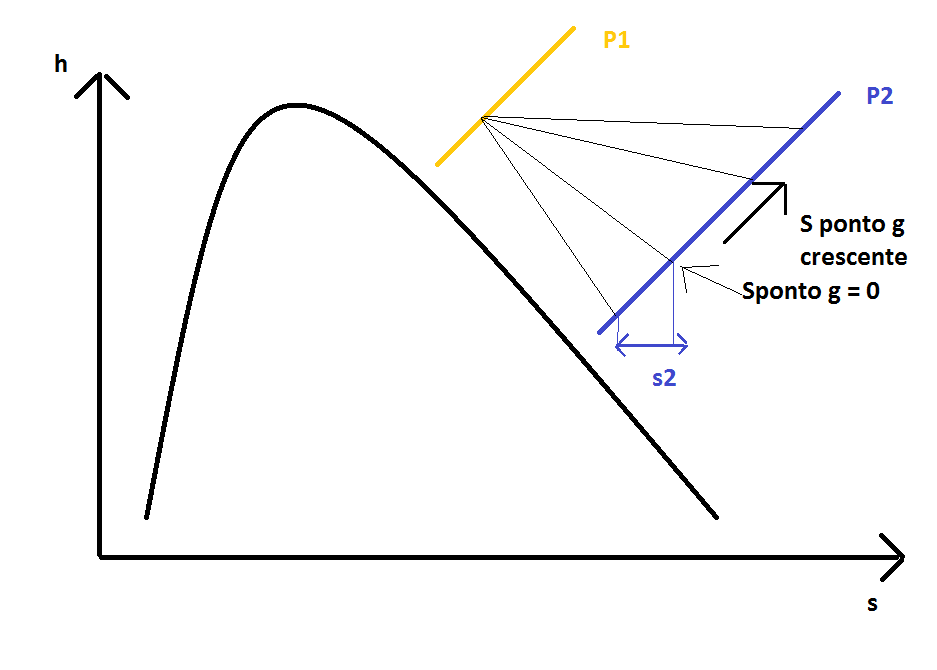
\includegraphics[scale=0.39]{./fig/2.png}
\caption{\label{fig:2}Diagrama de esforços solicitantes} 
\end{center}
\end{figure}

\begin{figure}[h]
\begin{center}
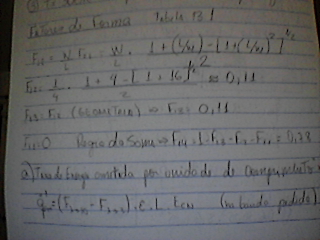
\includegraphics[scale=0.38]{./fig/3.png}
\caption{\label{fig:3}M = $\sqrt{58.3^{2}+12.1^{2}}=59.5Nm$} 
\end{center}
\end{figure}

Apesar dos momentos máximos atuarem no meio do comprimento da engrenagem, a favor da segurança vamos assumir que esses esforços se encontram na região de concentraçao de tensão.

 Acabamento superficial retificado
\[ \sigma _{t}  = 630 MPa\]
\[ \sigma _{y}  = 420 MPa\]

\[\sigma \footnote{variável} = \frac{32M}{\pi d^{3}}K_{\sigma}\]
\[\tau \footnote{constante} = \frac{16T}{\pi d^{3}}\]

\[k_{t,\tau}=2.0\ \ \ \ \ \ \ \ \ q = 0.9\]
\[k_{\tau}=1+(2-1)*0.9=1.9\]

\[\sigma_{a}=\frac{32*59.5*10^{3}*1.9}{\pi * 20^{3}} = 143.5Mpa\]

\[\tau _{m} = \frac{16*95*10^{3}}{\pi * 20^{3}}=60,5Mpa\]

\[(\frac{\eta \sigma_{a}}{\sigma_{fp}})^{2}+(\frac{\eta \sigma_{m}}{\sigma_{y}})^{2}=1\]

\begin{figure}[h]
\begin{center}
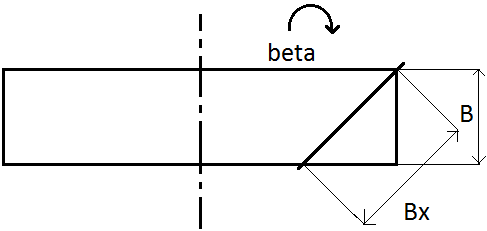
\includegraphics[scale=0.28]{./fig/4.png}
\caption{\label{fig:4}4} 
\end{center}
\end{figure}

$\eta$ = fator de segurança

\[\sigma_{eq a}= \sigma _{a} = 143.5 Mpa\]
\[\sigma_{eq m}= \sqrt{\sigma_{m}^{2}+3\tau_{m}^{2}}=\sqrt{1.8^{2}+3*60.5^{2}}=105 Mpa\]

\begin{table}[htbp]
  \centering
 % \caption{Add caption}
    \begin{tabular}{rr}
    \toprule
    Conf. & Kconf \\
    \midrule
    80\%  & 1 \\
    90\%  & 0.897 \\
    99\%  & 0.814 \\
    99.9\% & 0.753 \\
    \bottomrule
    \end{tabular}%
  \label{tab:1}%
\end{table}%

\[\sigma _{fp}=198 MPa\]

\begin{figure}[h]
\begin{center}
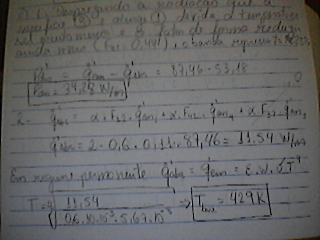
\includegraphics[scale=0.28]{./fig/6.png}
\caption{\label{fig:5}5} 
\end{center}
\end{figure}

\[k_{tam} = \left\lbrace (d*7.62)^{-0.107};2.80<=d_{1}<=51mm \right\rbrace \]  
\[k_{tam} = \left\lbrace  1.51*d^{-0.157};d>51mm \right\rbrace \]



\[\sigma _{eq,a}=\sigma_{a}=143.5MPa\]
\[\sigma _{eq,m}=\sqrt{3}\tau_{m}=104.8MPa\]
\[\sigma _{fp}= \sigma _{f}k_{os}k_{conf}k_{tam}k_{\theta}=\frac{\sigma}{2}*0.86*0.814*0.9*1\]

\[\eta ^{2}[(\frac{143.5}{198})^{2}+(\frac{104.8}{420})^{2}]=1\]
\[\eta^{2}=1.7\]
\[\eta = 1.3\]

\subsection*{Soderberg}

\[\eta\frac{\sigma _{a}}{\sigma _{fp}}+\eta\frac{\sigma _{m}}{\sigma _{y}}=1\]
\[\eta = 1.04\]

Hipótese:

\[\sigma _{a}=\frac{32M_{e}}{\pi d^{3}}K_{\sigma}\]
\[\tau _{a}= \frac{16T_{a}}{\pi d^{3}}K_{\tau}\]
\[\sigma _{m}=\frac{32M_{m}}{\pi d^{3}}\]
\[\tau _{m}= \frac{16T_{m}}{\pi d^{3}}\]

n=600 rpm, m = 10 kg, e = 1mm

\paragraph*{engrenagem desbalanceada}

\[\sigma _{db}=\frac{32M_{db}}{\pi d^{3}}=1.8 MPa\]
\[\sigma _{eq,m}=\sqrt{3\tau _{m}^{2}+\sigma _{m}^{2}}=10.5 MPa\]

\begin{figure}[h]
\begin{center}
\includegraphics[scale=0.48]{./fig/7.png}
\caption{\label{fig:7}$F_{c}=m\omega ^{2}e=10*63^{2}*1*10^{-3}=40N$} 
\end{center}
\end{figure}

\begin{figure}[h]
\begin{center}
\includegraphics[scale=0.48]{./fig/8.png}
\caption{\label{fig:8}Diagrama de Momento} 
\end{center}
\end{figure}

\newpage

Assumindo agora:

\[\frac{\sigma _{a}}{\sigma _{fp}}+\frac{\sigma _{m}}{\sigma _{y}}=\frac{1}{\eta}\]

\paragraph*{Hipótese}
\begin{itemize}
\item $\sigma$ flexão
\item $\tau$ torção
\end{itemize}

\begin{figure}[h]
\begin{center}
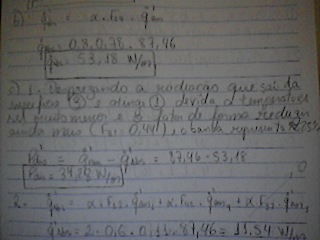
\includegraphics[scale=0.28]{./fig/5.png}
\caption{\label{fig:6}Hipóteses de flexão e torção} 
\end{center}
\end{figure}

\[\sigma _{eq,a} = \sqrt{\sigma _{a}^{2}+3\tau _{a}^{2}}\]
\[\sigma _{eq,m} = \sqrt{\sigma _{m}^{2}+3\tau _{m}^{2}}\]
\[\sigma _{a}=\frac{32M_{a}}{\pi d^{3}}k_{\tau}\]
\[\tau _{a}=\frac{16T_{a}}{\pi d^{3}}k_{\tau}\]

\[\sigma _{eq,a}=\frac{16}{\pi d^{3}}\sqrt{4M_{a}^{2}k_{\tau}^{2}+3T_{a}^{2}k_{\tau}^{2}}\]

\[\sigma _{eq,m}=\frac{16}{\pi d^{3}}\sqrt{4M_{m}^{2}k_{\tau}^{2}+3T_{m}^{2}k_{\tau}^{2}}\]

\[\frac{16}{\pi d^{3}}\left[\frac{ \sqrt{4M_{a}^{2}k_{\tau}^{2}+3T_{a}^{2}k_{\tau}^{2}}}{\sigma _{fp}}  +  \frac{\sqrt{4M_{m}^{2}k_{\tau}^{2}+3T_{m}^{2}k_{\tau}^{2}}}{\sigma _{y}} \right] = \frac{1}{\eta}\]
\\

Com $\eta$ = $1.5$, pelo critério de Soderberg

\[d = \left[\frac{16}{\pi }\left(\frac{ \sqrt{4M_{a}^{2}k_{\tau}^{2}+3T_{a}^{2}k_{\tau}^{2}}}{\sigma _{fp}}  +  \frac{\sqrt{4M_{m}^{2}k_{\tau}^{2}+3T_{m}^{2}k_{\tau}^{2}}}{\sigma _{y}} \right)\right]^{\frac{1}{3}}\]

\paragraph*{ASME}
\[d = \left[\left( \frac{16}{\pi } \right)^{2} \left(  \left( \frac{ \sqrt{4M_{a}^{2}k_{\tau}^{2}+3T_{a}^{2}k_{\tau}^{2}}}{\sigma _{fp}} \right)^{2}  +  \left( \frac{\sqrt{4M_{m}^{2}k_{\tau}^{2}+3T_{m}^{2}k_{\tau}^{2}}}{\sigma _{y}} \right)^{2}  \right)\right]^{\frac{1}{6}}\]

Fórmulas de WestingHouse para cálculo de eixo


\end{document}